% !TEX root = ../Thesis.tex
\chapter{Encoding}\label{Encoding}
As introduced in \ref{DIMACS}, the SAT-Solvers expect a DIMACS file as input that describes a set of clauses. This chapter details how the different Sudoku Variants and their rules can be encoded into these clause sets. We elaborate on the different variants separately, but as long as there are no direct contradictions, the different variants and rules could be freely combined (which can be done by creating the union of the corresponding clause sets). In the following formulae, we use the notation $s_{x_{n},...,x_{0}}$ to describe boolean variables, the corresponding integer numbers in the DIMACS files have the values $x_{n}*10^{n}+...+x_{0}*10^{0}$. For example, the literal $\neg s_{1,2,3}$ would be transformed to $-123$. There are two ways how we choose the name (number) for a variable during the encoding process:

\begin{enumerate}
    \item We use increasing values starting from 1. These dynamically chosen values are, by example, used for variables necessary to encode PBCs. We use $s_{v}$, for $v \in \mathbb{N}$, to describe them in the formulae as we do not know the corresponding integers in advance.
    \item  We use fixed intervals of numbers to encode certain constraints. Here every digit of a number has a semantic meaning. The dynamically generated variables skip these fixed intervals. For example, a fixed interval is used for the boolean variables that describe the cell values of the Sudoku grid. The variable $s_{x,y,z}$ is true if and only if cell ($x$,$y$) has the value $z$ assigned (as proposed in \cite{Lynce2006SudokuAsASATProblem}). The other used fixed intervals are indicated in the corresponding subsections of this chapter\todo{Actually do that!}. 
\end{enumerate}

It is important to note that the numbers used as variable names are not ``continuous". There are ``gaps". For example, not all integers from 1 to 1000 are used. This is because the dynamic variables skip the entire interval from 111 to 999, and the fixed variables used to encode cell values will not use numbers like 400 because we start to count rows at 1, and the grid cells can only hold values from 1 to 9. The needed fixed intervals grow larger when encoding more complicated variants, and with them often also the ``gaps". These gaps have no effect logically, but they can have a non-negligible effect on the time needed by the solvers, which is affected by the highest integer value used to describe a variable. However, as the ``gaps" are the same when encoding Sudokus with the same rules, they should not make a difference when comparing solver-times.

\section{Encoding of PBCs using Binary Decision Diagrams}\label{PBCEncodingBDD}
A binary decision diagram (BDD) is a directed graph that can be used to represent logical formulae. Every graph node corresponds to a partial assignment to the variables in the formula. The BDD has a root node which corresponds to the empty assignment. Every edge from a node $u$ to a node $v$ corresponds to an extension of the assignment of node $u$. Every node has at most two successors, one reachable via the edge that corresponds to assigning $true$ and one via the edge that corresponds to assigning $false$ to the next variable. Nodes store references to their successors as \emph{$true_{child}$} and \emph{$false_{child}$} respectively. Variables are considered in a fixed order. As recommended in \cite{Een2006TranslatingPC}, ordering them by decreasing\todo{do that} weight values is generally reasonable. If the variable value assignment determines the value of the entire logical formula that the BDD represents, the corresponding successor is a terminal node. Terminal nodes have no successors, as their corresponding assignment already satisfies the  logical formula, or it is impossible to extend the  assignment to satisfy the formula (The assignment of terminal nodes does not have to be a total one).\\

Since we want to encode PBCs, it is helpful to store for each node the sum that is achieved by adding together all the weights of the variables assigned to $true$ by the (partial) assignment of the node. Also, we assign an integer number to each node which can later be used to describe a boolean variable (called \emph{assignmentVariable}) that is true if and only if the partial assignment of the node is present.\todo{``present" is not correct...formulate it better...} \\

The BDD can be built using a Breadth-First-Search starting in the root, shown as pseudocode in \ref{CodeBDDConstruction}. The version we use for encoding PBCs differs from the one introduced in \cite{Een2006TranslatingPC} because it is written to encode equations rather than inequations. Further, the used queue has additional functionalities: Given a node, it can check if it already contains a node with the same attribute values and can return said equal node. The \emph{updated sums} of successor nodes either are the same as their predecessors ($false$ was assigned) or are equal to the sum of their predecessor plus the weight value corresponding to the edge that led to them (true was assigned).



{
\lstset%
{%
    emph=[1]%
    {%
        If,
        While,
        Else,
    },
    emphstyle=[1]{\bfseries},
    %
    emph=[2]% Variable Types
    {% 
       false,
       true,
    },
  emphstyle=[2]{\textit{}\ttfamily},
}
\begin{lstlisting}[frame=single,caption={Pseudo Code of BDD construction},captionpos=b, label=CodeBDDConstruction]
queue.append(root)
While not queue is empty:
    Node current = queue.poll()
    If assigning next variable leads to a total assignment:
        Node cT = Create true successor node with updated sum
        Node cF = Create true successor node with updated sum
    Else:
        Node cT = Create true successor node with updated sum
        If cT.sum >= RHS:
            # true successor is a terminal node
        Else:
            # true successor is not a terminal node
            If cT not in queue:
                queue.append(cT)
            Else:
                cT = queue.get(cT)
        Node cF = Create false successor node with updated sum
        If cF.sum + sum of remaining weights < RHS:
            # false successor is a terminal node
        Else:
            # false successor is not a terminal node
            If cF not in queue:
                queue.append(cF)
            Else:
                cF = queue.get(cF)
    current.true_child = cT
    current.false_child = cF
\end{lstlisting}
}

Once the BDD is built, we can transform it into clauses. In \cite{Een2006TranslatingPC}, it is explained how this can be achieved by treating the BDD network as a circuit of ITEs (if-then-else gates). However, it suffices to know that the BDD can be transformed by doing a second Breadth-First-Search starting from the root and that for each visited node that is not a terminal node, the following six implications must be added to the set of formulas:

\begin{enumerate}
    \item If the \emph{assignmentVariable} of the current node is true and the variable corresponding to the leaving edges from this node is true, then it follows that the \emph{assignmentVariable} of the $true_{child}$ node is true.
    \item If the \emph{assignmentVariable} of the current node is true and the variable corresponding to the leaving edges from this node is false, then it follows that the \emph{assignmentVariable} of the $false_{child}$ node is true.
    \item If the \emph{assignmentVariable} of the current node is false and the variable corresponding to the leaving edges from this node is true, then it follows that the \emph{assignmentVariable} of the $true_{child}$ node is false.
    \item If the \emph{assignmentVariable} of the current node is false and the variable corresponding to the leaving edges from this node is false, then it follows that the \emph{assignmentVariable} of the $false_{child}$ node is false.
    \item If the \emph{assignmentVariable} of the $true_{child}$ node is true and the \emph{assignmentVariable} of the $false_{child}$ node is true, then it follows that the \emph{assignmentVariable} of the current node is true.
    \item If the \emph{assignmentVariable} of the $true_{child}$ node is false and the \emph{assignmentVariable} of the $false_{child}$ node is false, then it follows that \emph{assignmentVariable} of the current node is false.
\end{enumerate}

Additionally, we add a clause that only contains the positive literal corresponding to the \emph{assignmentVariable} of the root node. Also, when visiting a node during this second Breadth-First-Search, we only append its children that are not terminal nodes. For children that are terminal nodes, we add a clause to the set of clauses: 
\begin{itemize}
    \item If the child's sum is equal to the RHS, a clause containing a positive literal corresponding to the \emph{assignmentVariable} of the child is added.
    \item If the child's sum is unequal the RHS, a clause containing a negative literal corresponding to the \emph{assignmentVariable} of the child is added.
\end{itemize}
An example is shown in Figure \ref{fig:BDDExample} where the BDD and the clauses are depicted that are used to encode the PBC $6*v_1+4*v_2+2*v_3=6$. The already achieved sums are written inside the nodes and the nodes \emph{assignmentVariables} are denoted as $a_i$ for $i\in \{1,2,3,4,5,6,7\}$. Edges with a circle are assigning $false$. Edges with a line are assigning $true$.

\begin{figure}
\centering
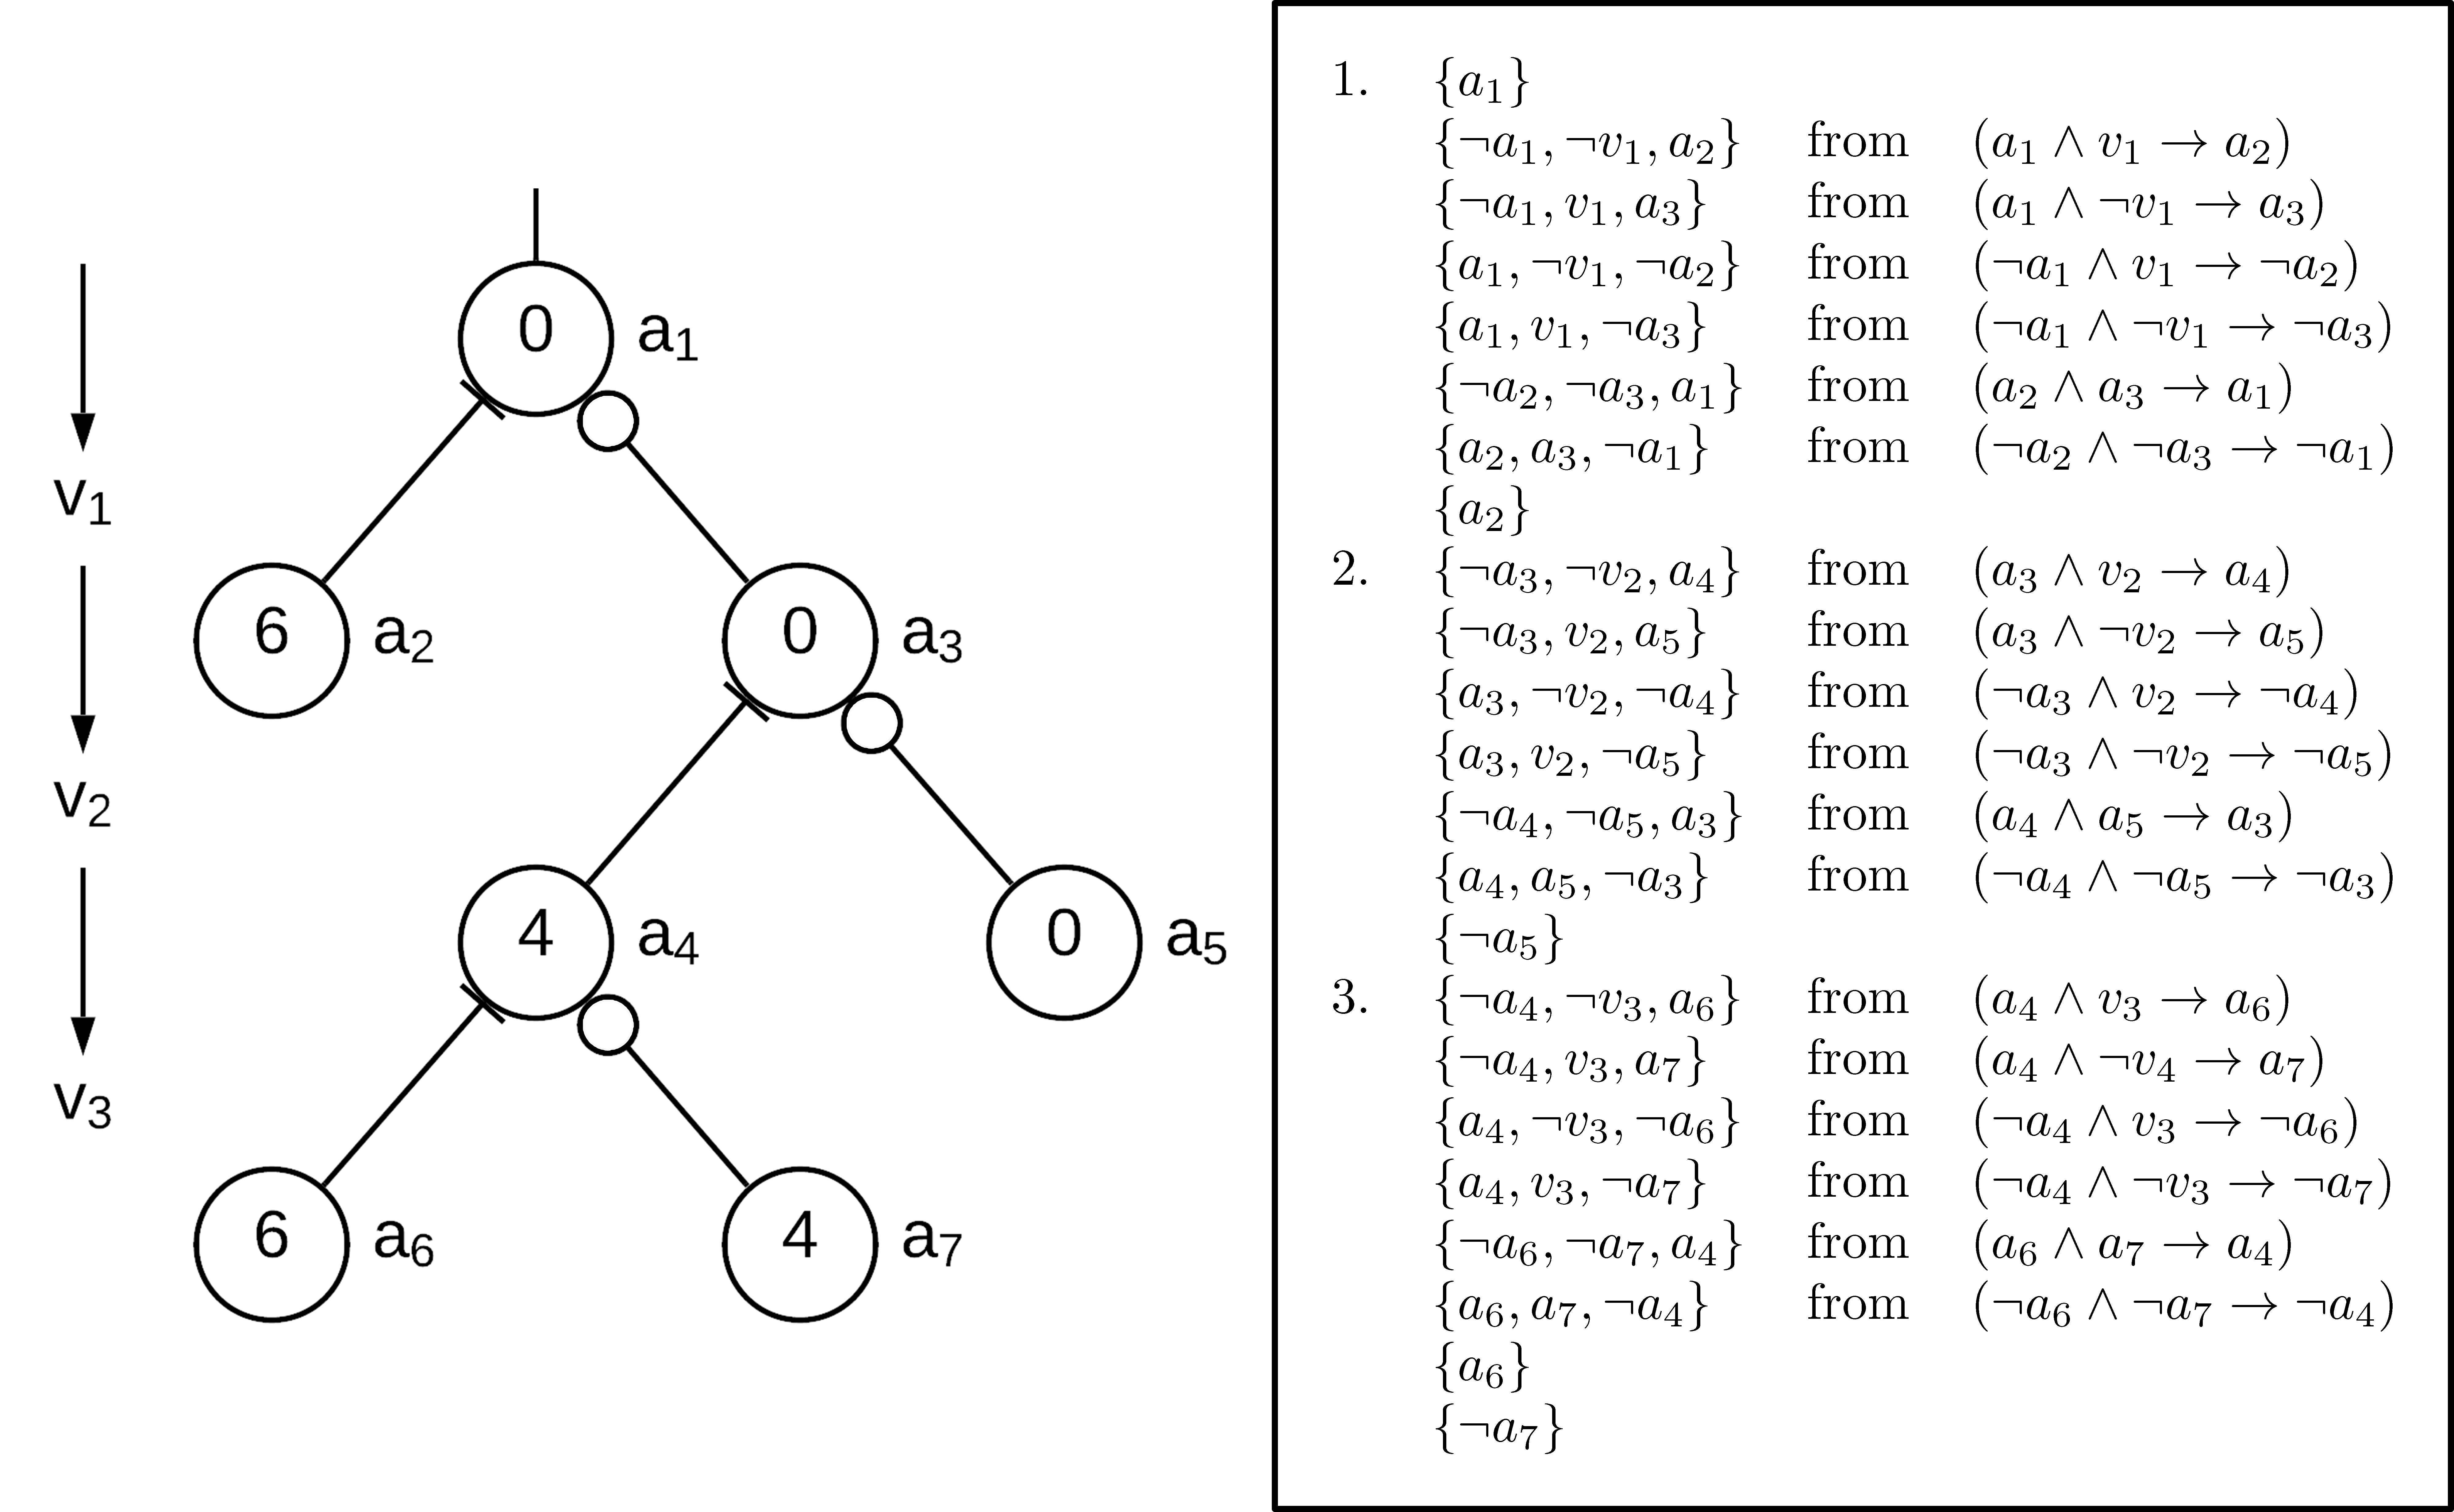
\includegraphics[width=\textwidth]{Figures/BDDExampleComposition.png}
\caption{BDD and clauses to encode $6*v_1+4*v_2+2*v_3=6$}
\label{fig:BDDExample}
\end{figure}


\section{Encoding of PBCs using Adder-Networks}\label{PBCEncodingAdderNetworks}

\section{Encoding of Sudoku Variants and Constraints}

\subsection{Normal Sudoku}
The normal Sudoku rules as introduced in \ref{NormalSudoku} can be broken down into the following five constraints, which can be encoded into clauses. The following encoding can be seen as a direct encoding using at-least-one and at-most-one clauses and was proposed by \cite{Lynce2006SudokuAsASATProblem} where it is called the minimal encoding:\\


\begin{table}[h!]
    \centering
    \begin{tabular*}{\textwidth}{l @{\extracolsep{\fill}}  c  c}
        \hline
        \\
        Constraint & Formula & \#Clauses\\
        \\
        \hline
        \\
        At least one number from 1 to 9 appears in each grid cell. & (S-\ref{S-i}) & 81\\
        \\
        Every number appears at most once per row. & (S-\ref{S-ii}) & 2916\\
        \\
        Every number appears at most once per column. & (S-\ref{S-iii}) & 2916\\
        \\
        Every number appears at most once per box. & (S-\ref{S-iv}) and (S-\ref{S-v}) & 2916\\
        \\
        Every cell that contains a hint can only have that value. & (S-\ref{S-vi}) & 1/hint\\
        \\
        \hline
    \end{tabular*}
        \caption{Constraints of Normal Sudoku.}
    \label{tab:NormalSudoku}
\end{table}


Formulae of clauses:\todo{Are "And" operators needed in last formula?}\\
\begin{tabular*}{\textwidth}{ l @{\extracolsep{\fill}} c}
    \\
    $\displaystyle \bigwedge_{x=1}^9 \bigwedge_{y=1}^9 \bigvee_{z=1}^9 s_{x,y,z}$  & \consCount{S} \label{S-\roman{cons}}\\
    \\
    $\displaystyle \bigwedge_{y=1}^9 \bigwedge_{z=1}^9 \bigwedge_{x=1}^9 \bigwedge_{i=x+1}^9 \neg s_{x,y,z} \lor \neg s_{i,y,z}$  & \consCount{S} \label{S-\roman{cons}}\\
    \\
    $\displaystyle \bigwedge_{z=1}^9 \bigwedge_{x=1}^9 \bigwedge_{y=1}^9 \bigwedge_{i=y+1}^9 \neg s_{x,y,z} \lor \neg s_{x,i,z}$  & \consCount{S} \label{S-\roman{cons}}\\
    \\
    $\displaystyle \bigwedge_{z=1}^9 \bigwedge_{i=0}^2 \bigwedge_{j=0}^2 \bigwedge_{x=1}^3 \bigwedge_{y=1}^3 \bigwedge_{k=y+1}^3 \neg s_{(3*i+x),(3*j+y),z} \lor \neg s_{(3*i+x),(3*j+k),z}$  & \consCount{S} \label{S-\roman{cons}}\\
    \\
    $\displaystyle \bigwedge_{z=1}^9 \bigwedge_{i=0}^2 \bigwedge_{j=0}^2 \bigwedge_{x=1}^3 \bigwedge_{y=1}^3 \bigwedge_{k=x+1}^3 \bigwedge_{l=1}^3 \neg s_{(3*i+x),(3*j+y),z} \lor \neg s_{(3*i+k),(3*j+l),z}$  & \consCount{S} \label{S-\roman{cons}}\\
    \\
    $s_{x,y,input_{x,y}}$,  for every $(x,y)$ s.t. input$_{x,y}$ $\neq 0$  & \consCount{S} \label{S-\roman{cons}}\\
\end{tabular*}\\

    
\subsection{Anti-Knight}
To encode the Anti-Knight rule, one must ensure that for each grid cell (x,y), it is forbidden to have the same value as its neighbours. The term neighbour of a cell (x,y) here corresponds to the cells that are one knight distance away from it. The set of neighbours to cell (x,y) can be defined as:\\ $N(x,y) = \{(i,j)~|\texttt{ cell }(i,j) \texttt{ one knight distance from cell }(x,y)\}$.
\begin{table}[h!]
    \centering
    \begin{tabular*}{\textwidth}{l @{\extracolsep{\fill}} c  c}
        \hline
        \\
        Constraint & Formula & \#Clauses\\
        \\
        \hline
        \\
        \makecell[cl]{Cells that are one knight-distance apart (neighbours) \\ must have different values.} & (AK-\ref{AK-i}) & 2016\\
        \\
        \hline
    \end{tabular*}
        \caption{Constraints of Anti-Knight rule.}
    \label{tab:AntiKnight}
\end{table}


Formula of clauses:\\
\begin{tabular*}{\textwidth}{ l @{\extracolsep{\fill}} c}
    $\displaystyle \bigwedge_{x=1}^9 \bigwedge_{y=1}^9 \bigwedge_{(i,j)\in N(x,y)} \bigwedge_{z=1}^9 \neg s_{x,y,z} \lor \neg s_{i,j,z}$ &\consCount{AK} \label{AK-\roman{cons}}\\\
\end{tabular*}\\

\newpage
\subsection{Killer}
\paragraph{Using PBCs:} For every killer cage of the input, we create a list of its cells. From every list, a PBC is created as follows: For every cell (x,y) of a cage, we add $\sum_{i=1}^{9} (s_{x,y,i}*i)$ to the left-hand side of the PBC. The right-hand side of the PBC is set to the target sum that was given as input. The different PBCs (one for every killer cage) can then be encoded into clauses, as explained in \ref{PBCEncodingBDD} and \ref{PBCEncodingAdderNetworks}.

\paragraph{Using PBCs + Combinations:}
The PBC approach can be further optimized, because given a fixed number of summands not all values from 1 to 9 can be used to achieve a certain sum. In example if a cage has a target sum of 8 and consists of three cells, the number of possible value combinations to achive the target sum is fairly limited. There are only two possible value combinations $1+2+5=8$ and $1+3+4=8$, so the allowed values that the cells could take are 1, 2, 3, 4 and 5. When constructing the PBC this knowladge can be used to reduce the number of variable-value products on the left hand side of the equation. For every cell in a cage we only add the variable times the corresponding value (to the left hand side) if the value is an allowed one.

\paragraph{Using Combinations:}
Another possibility is to completely abandon PBCs and exploit that only certain value combinations are possible given a cage with a fixed target sum and fixed number of cells that belong to it. To encode this every combination is given a corresponding variable $varNum$ which is true iff the corresponding combination is used in a certain cage. This can then be encoded in the following way:\\

\begin{table}[h!]
    \centering
    \begin{tabular*}{\textwidth}{l @{\extracolsep{\fill}} c}
        \hline
        \\
        Constraint & Formula\\
        \\
        \hline
        \\
        \makecell[cl]{For every Cage $g$ and possible combination $c$ (for that \\
        cage) it holds that, either the cage's target sum is not \\
        achieved using combination $c$ or every cage cell \\
        contains at least one value of the combination.} & (K-\ref{K-i})\\
        \\
        In every Cage $g$ at least one combination $c_a$ is used. & (K-\ref{K-ii})\\
        \\
        In every Cage $g$ at most one combination $c_a$ is used. & (K-\ref{K-iii})\\
        \\
        \makecell[cl]{Every value from 1 to 9 appears at most once within \\
        the cells of a cage.} & (K-\ref{K-iv})\\
        \\
        \hline
    \end{tabular*}
        \caption{Constraints of Killer Sudoku rules.}
    \label{tab:Killer}
\end{table}

\newpage
Formulae of clauses:\\
\begin{tabular*}{\textwidth}{ l c @{\extracolsep{\fill}} c}
    \\
    $\displaystyle \bigwedge_{g:groups} \bigwedge_{c:combis_g} \bigwedge_{[x,y]:g} -s_v \lor \bigvee_{z:c}  s_{x,y,z}$ & & \consCount{K} \label{K-\roman{cons}}\\
    \\
    $\displaystyle \bigwedge_{g:cages} \bigvee_{a=1}^{\#combis_g} varNum_{a}$ & & \consCount{K} \label{K-\roman{cons}}\\
    \\
    $\displaystyle \bigwedge_{g:cages} \bigwedge_{a=1}^{\#combis_g} \bigwedge_{b=a+1}^{\#combis_g} \neg varNum_a \lor \neg varNum_b$  & & \consCount{K} \label{K-\roman{cons}}\\
    \\
    $\displaystyle \bigwedge_{g:cages} \bigwedge_{[x_i,y_i]:g} \bigwedge_{[x_j,y_j]:g} \bigwedge_{z=1}^{9} \neg x_i y_i z \lor \neg x_j y_j z$ & with $[x_i,y_i] \neq [x_j,y_j]$ &\consCount{K} \label{K-\roman{cons}}\\
\end{tabular*}\\

